\ylDisplay{Traat} % Ülesande nimi
{Jaan Kalda} % Autor
{lõppvoor} % Voor
{2008} % Aasta
{G 7} % Ülesande nr.
{5} % Raskustase
{
% Teema: Elektriahelad
\ifStatement
Ühtlase ristlõikega traati (ristlõike pindala $S = \SI{1}{mm^2}$) venitati nii, et tema erinevad lõigud venisid erinevalt. Enne venitamist oli traadile märgitud jooned iga millimeetri tagant. Joonisel on toodud nende joonte vahekaugused $\Delta$ pärast venitamist sõltuvuses kaugusest traadi ühest otsast $l$ ($l$ on mõõdetud pärast venitamist). Leidke selle nüüdseks 4 meetri pikkuse traadi takistus, arvestades, et traadi materjali tihedus ja eritakistus $\rho = \SI{1e-6}{\ohm.m}$ venitamise tagajärjel ei muutunud.

\begin{center}
	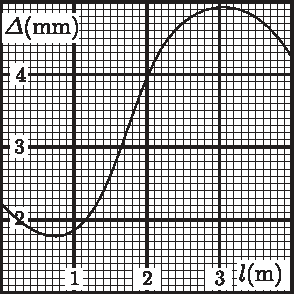
\includegraphics[width=0.6\linewidth]{2008-v3g-07-yl}
\end{center}
\fi


\ifHint
Kõigepealt tasub leida lühikese traadijupi takistus ning seejärelt üritada saadud avaldist summeerida terve traadi ulatuses.
\fi


\ifSolution
Traadijupp pikkusega $\delta$ omab ristlõikepindala $s = S \cdot \SI{1}{mm}/\Delta$ ning takistust $r = \rho \delta /s = \rho \delta \Delta \cdot \SI{1}{mm^{-3}}$. Liites kokku kõikide väikeste juppide takistused näeme, et kogutakistus $R = \rho A \cdot \SI{1}{mm^{-3}}$ , kus $A$ on graafiku alune pindala (liita tuleb ka joonest $\Delta = \SI{1}{mm}$ allapoole jääv osa). Joonise abil leiame $A \approx \SI{14}{mm\cdot m}$ ning seega $R \approx \SI{14}{\ohm}$. 
\fi
}